\documentclass[table]{article}
% For math environments
\usepackage{amsmath, amsfonts}
% For links
\usepackage[colorlinks=true,
    linkcolor = blue,
    urlcolor  = blue,
    citecolor = blue,
    anchorcolor = blue]{hyperref}
% Put space between paragraphs
\usepackage{parskip}
% For figures
\usepackage{tikz}
% Set the margins to not be ridiculous
\usepackage[margin=0.75in]{geometry}
% For multiple columns
\usepackage{multicol}
% For controlling enum/itemize spacing and indentation
\usepackage{enumitem}
% More math symbols
\usepackage{amssymb}
% To change enumerate labels

% For tikz plots
\usepackage{pgfplots}
% This isn't needed but avoids a compiler warning
\pgfplotsset{compat=1.16}

% Allow multi-line equations to be broken across pages
\allowdisplaybreaks

% Use @ as a letter
\makeatletter

% Scale down all tikz coordinates while maintaining font size
\tikzset{every picture/.style={scale=0.45, every picture/.style={}}}


% Macros
% Monospace code
\def\code#1{\texttt{#1}}

% Greek letters
\def\a{\alpha}
\def\b{\beta}
\def\g{\gamma}
\def\d{\delta}
\def\D{\Delta}

% Commands that make life easier
\newcommand\gath[1]{\begin{gather} #1 \end{gather}}
\newcommand\ali[1]{\begin{align} #1 \end{align}}
\newcommand\parens[1]{\left( #1 \right)}
\newcommand\squares[1]{\left[ #1 \right]}
\newcommand\braces[1]{\left\{ #1 \right\}}
\newcommand\angles[1]{\left\langle #1 \right\rangle}
\newcommand\deriv[2]{\frac{d #1}{d #2}}
\newcommand\abs[1]{\left| #1 \right|}
\newcommand\floor[1]{\left\lfloor #1 \right\rfloor}
\DeclareMathOperator{\lcm}{lcm}
\def\non{\nonumber \\}

% Multiline equation space
\def\mlesp{\hspace{1.2cm}}

% For grid diagrams
\newcommand\gridbox[3]{\draw (#1,#2) rectangle (#1+1,#2+1) node[pos=.5] {#3};}
\newcommand\gridboxh[3]{\draw[fill=red!20] (#1,#2) rectangle (#1+1,#2+1) node[pos=.5] {#3};}
\newcommand\gridboxb[3]{\draw[fill=black] (#1,#2) rectangle (#1+1,#2+1) node[pos=.5] {#3};}
\newcommand\gridsym[3]{\node at (#1+0.5,#2+0.5) {$#3$};}
\newcommand\gridblank[2]{\filldraw[draw=gray, color=gray] (#1,#2) rectangle (#1+1,#2+1);}
\newcommand\gridcirc[2]{\draw (#1 + 0.5,#2 + 0.5) circle (0.25);}
\newcommand\cwlab[3]{
  \def\dd{0.15}
  \draw (#1 + \dd - 0.03, #2 + 1 - \dd) node {\scriptsize #3};
}

\def\bbw{3.5}
\def\bbh{2}
\newcommand\bigbox[3]{\draw (#1*\bbw,#2*\bbh) rectangle (#1*\bbw+\bbw,#2*\bbh+\bbh) node[pos=.5] {#3};}
\newcommand\bbtextr[3]{\node[right] at (#1*\bbw,#2*\bbh+0.5*\bbh) {#3};}
\newcommand\bbtextb[3]{\node[align=center] at (#1*\bbw+0.5*\bbw,#2*\bbh+0.5*\bbh) {#3};}

% Box puzzle stock answer
\newcommand\boxans[1]{
  Logic was used to deduce the solution:

  #1

  This was verified using Python as well as shown to be unique with a brute force approach.
}

% Multiple numbers
\newcommand\mn[1]{$#1$'s}

% Commands for problems
\newcommand\problem[4]{
  \section*{#1}

  Question: #3
  
  Answer: #2
  
  Explanation: #4
}
\newcommand\aproblem[4]{\problem{Dec #1}{#2}{#3}{#4}}
\newcommand\cproblem[4]{\problem{Problem #1}{#2}{#3}{#4}}

\def\advent@xxiv@i{
  Eve writes down five different positive integers.
  The sum of her integers is $16$. What is the product of her integers?
}

\def\advent@xxiv@ii{
  $14$ is the smallest even number that cannot be obtained by rolling two $6$-sided dice and finding the product of the numbers rolled.

  What is the smallest even number that cannot be obtained by rolling one hundred $100$-sided dice and finding the product of the numbers rolled?
}

\def\advent@xxiv@iii{
  There are $5$ ways to write $5$ as the sum of positive odd numbers:
  \begin{itemize}
    \item $1 + 1 + 1 + 1 + 1$
    \item $1 + 1 + 3$
    \item $3 + 1 + 1$
    \item $1 + 3 + 1$
    \item $5$
  \end{itemize}

  How many ways are there to write $14$ as the sum of positive odd numbers?
}

\def\advent@xxiv@iv{
  The geometric mean of a set of $n$ numbers is computed by mulitplying all the numbers together, then taking the $n$th root.
  The factors of $9$ are $1$, $3$, and $9$.
  The geometric mean of these factors is
  \gath{
    \sqrt[3]{1 \times 3 \times 9} = \sqrt[3]{27} = 3
  }
  What is the smallest number where the geometric mean of its factors is $13$?
}

\def\advent@xxiv@v{
  The sum of $11$ consecutive integers is $2024$.
  What is the smallest of the $11$ integers?
}

\def\advent@xxiv@vi{Put the digits 1 to 9 (using each digit exactly once) in the boxes so that the sums are correct. The sums should be read left to right and top to bottom ignoring the usual order of operations. For example, 4+3×2 is 14, not 10. Today's number is the product of the numbers in the red boxes.
  The number $n$ has $55$ digits.
  All of its digits are $9$.
  What is the sum of the digits of $n^3$?
}

\def\advent@xxiv@vii{
  What is the obtuse angle in degrees between the minute and hour hands of a clock at 08:22?
}

\def\advent@xxiv@viii{
  It is possible to arrange $4$ points on a plane and draw non-intersecting lines between them to form $3$ non-overlapping triangles:

  \begin{center}
    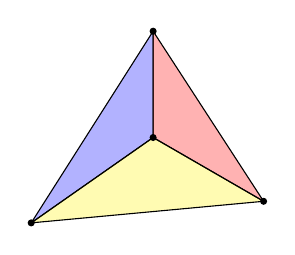
\begin{tikzpicture}
      \def\ds{3}
      \def\pa{(0: 0)}
      \def\pb{(90: \ds)}
      \def\pc{(215: 1.4*\ds)}
      \def\pd{(-30: 1.2*\ds)}

      \def\bcr{3}
      \def\scr{0.55*\bcr}
      \def\sca{34}
      \def\mcr{0.7*\bcr}
      \def\mca{142}
      \def\pr{0.1}

      % Triangles
      \draw[fill=blue,fill opacity=0.3] \pa -- \pb -- \pc -- cycle;
      \draw[fill=red,fill opacity=0.3] \pa -- \pb -- \pd -- cycle;
      \draw[fill=yellow,fill opacity=0.3] \pa -- \pd -- \pc -- cycle;

      % Points
      \fill \pa circle (\pr);
      \fill \pb circle (\pr);
      \fill \pc circle (\pr);
      \fill \pd circle (\pr);
    \end{tikzpicture}
  \end{center}

  It is not possible to make more than $3$ triangles with $4$ points.

  What is the maximum number of non-overlapping triangles that can be made by arranging $290$ points on a plane and drawing non-intersecting lines between them?
}

\def\advent@xxiv@ix{
  Put the digits $1$ to $9$ (using each digit exactly once) in the boxes so that the sums are correct.
  The sums should be read left to right and top to bottom ignoring the usual order of operations.
  For example, $4 + 3 \times 2$ is $14$, not $10$.
  Today's number is the product of the numbers in the red boxes.

  \grid@advent@xxiv@ix{}{}{}{}{}{}{}{}{}
}

\def\advent@xxiv@x{
  A number is a palindrome if it's the same when its digits are written in reverse order.

  What is the sum of all the numbers between $10$ and $100$ that are palindromes?
}

\def\advent@xxiv@xi{
  There are $6$ sets of integers between $1$ and $5$ (inclusive) that contain an odd number of numbers whose median value is $3$:

  \begin{itemize}
    \item $\braces{3}$
    \item $\braces{1,3,4}$
    \item $\braces{2,3,4}$
    \item $\braces{1,3,5}$
    \item $\braces{2,3,5}$
    \item $\braces{1,2,3,4,5}$
  \end{itemize}

  How many sets of integers between $1$ and $11$ (inclusive) are there that contain an odd number of numbers whose median value is $5$?
}

\def\advent@xxiv@xii{
  Holly picks a three-digit number.
  She then makes a two-digit number by removing one of the digits.
  The sum of her two numbers is $309$.
  What was Holly's original three-digit number?
}

\def\advent@xxiv@xiii{
  Today's number is given in this crossnumber.
  No number in the completed grid starts with $0$.

  \begin{multicols}{2}
    \crossnumstd{}{}{}{}{}{}{}{}{}

    \vfill\null
    \columnbreak

    \begin{center}
      \textbf{Across}

      \begin{tabular}{clc}
        \textbf{1} & Today's number.  & (\textbf{3}) \\
        \textbf{4} & Two times 5A.    & (\textbf{3}) \\
        \textbf{5} & A multiple of 1. & (\textbf{3})
      \end{tabular}

      \textbf{Down}

      \begin{tabular}{clc}
        \textbf{1} & Sum of digits is 15. & (\textbf{3}) \\
        \textbf{2} & Sum of digits is 19. & (\textbf{3}) \\
        \textbf{3} & Three times 5A.      & (\textbf{3})
      \end{tabular}
    \end{center}
  \end{multicols}
}

\def\advent@xxiv@xiv{
  $15^3$ is $3375$.
  The last $3$ digits of $15^3$ are $375$.

  What are the last $3$ digits of $15^{1234567890}$?
}

\def\advent@xxiv@xv{
  The number $2268$ is equal to the product of a square number (whose last digit is not $0$) and the same square number with its digits reversed: $36 \times 63$.

  What is the smallest three-digit number that is equal to the product of a square number (whose last digit is not $0$) and the same square number with its digits reversed?
}

\def\advent@xxiv@xvi{
  Put the digits $1$ to $9$ (using each digit exactly once) in the boxes so that the sums are correct.
  The sums should be read left to right and top to bottom ignoring the usual order of operations.
  For example, $4 + 3 \times 2$ is $14$, not $10$.
  Today's number is the product of the numbers in the red boxes.

  \grid@advent@xxiv@xvi{}{}{}{}{}{}{}{}{}
}

\def\advent@xxiv@xvii{
  The number $40$ has $8$ factors: $1$, $2$, $4$, $5$, $8$, $10$, $20$, and $40$.

  How many factors does the number $2^{26} \times 5 \times 7^5 \times 11^2$ have?
}

\def\advent@xxiv@xviii{
  TODO
}

\def\card@xxiv@i{
  What is the largest number you can make by using the digits $1$ to $4$ to make two $2$-digit numbers, then mutiplying the two numbers together?
}

\def\card@xxiv@ii{
  What is the largest number you can make by using the digits $0$ to $9$ to make a $2$-digit number and an $8$-digit number, then mutiplying the two numbers together?
}

\def\card@xxiv@iii{
  The expansion of $(2x+3)^2$ is $4x^2 + 12x + 9$.
  The sum of the coefficients of $4x^2 + 12x + 9$ is $25$.
  What is the sum of the coefficients of the expansion of $(30x + 5)^2$?
}

\def\card@xxiv@iv{
  What is the sum of the coefficients of the expansion of $(2x+1)^{11}$?
}

\def\card@xxiv@v{
  What is the geometric mean of all the factors of $41306329$?
}

\def\card@xxiv@vi{
  What is the largest number for which the geometric mean of all its factors is $92$?
}

\def\card@xxiv@vii{
  What is the sum of all the factors of $7^4$?
}

\def\card@xxiv@viii{
  How many numbers between $1$ and $28988500000$ have an odd number of factors?
}

\def\card@xxiv@ix{
  Eve found the total of the $365$ consecutive integers starting at $500$ and the total of the next $365$ consecutive integers, then subtracted the smaller total from the larger total.
  What was her result?
}

\def\card@xxiv@x{
  Eve found the total of the $n$ consecutive integers starting at a number and the total of the next $n$ consecutive integers, then subtracted the smaller total from the larger total.
  Her result was $22344529$.
  What is the largest possible value of $n$ that she could have used?
}


\begin{document}

\title{MS Scroggs Advent Calendar 2015 Answers}
\author{Dan Whitman}
\date{}

\maketitle

Answers: \href{https://www.mscroggs.co.uk/puzzles/advent2015}{https://www.mscroggs.co.uk/puzzles/advent2015}

\aproblem{1}{200}{\advent@xv@i}{
  In general, the largest area $n$-gon that will fit in a circle is a regular $n$-gon with a circumradius equal to the radius of the circle.
  Of course, a rectangle is a quadrilateral, that is a $4$-gon, so that the largest area rectangle will actually be a square with a diagonal equal to the diameter of the circle.
  A square with sides $s$ has an area $A = s^2$ and a diagonal of $d = \sqrt{2}s$ so that of course $s = d / \sqrt{2}$.
  We have a circle of radius $r = 10$ so that the diameter is of course $2r$.
  The area of the square is thus
  \gath{
    A = s^2 = \parens{\frac{d}{\sqrt{2}}}^2 = \frac{d^2}{2} = \frac{(2r)^2}{2} = \frac{4r^2}{2} = 2r^2 = 2 \cdot 10^2 = 200 \,,
  }
  which is our answer.
}

\aproblem{2}{154}{\advent@xv@ii}{
  Consider a twelve hour period from 12:01 to 12:01.
  The minute hand aligns with the hour hand first between 1:00 and 2:00 (precisely at 1:05), and then between 2:00 and 3:00 (at exactly 2:10), and lastly at exactly 12:00.
  This is $11$ times once the clock strikes the next 12:01.
  Hence during a day starting at 12:01 (i.e. two $12$ hour periods) this happens $22$ times.
  So, during a week, this happens $7 \cdot 22 = 154$ times.
}

\aproblem{3}{304}{\advent@xv@iii}{
  The answer is just from the blog post.
  Since the number exploits symmetry and the fact that games are ended once a player wins, deriving this number analytically or even using a Python program would be highly non-trivial.
}

\aproblem{4}{108}{\advent@xv@iv}{
  \boxans{\grid@advent@xv@iv{1}{9}{4}{2}{7}{5}{3}{8}{6}}
}

\aproblem{5}{208}{\advent@xv@v}{
  For a triangle to be valid, the pairwise sum of the lengths of two sides must be strictly greater than the third side.
  So suppose we have potential sides $a$, $b$, and $c$ such that
  \gath{
    0 < a \leq b \leq c \,. \label{eqn:05:ineq}
  }
  We always have
  \gath{
    b > 0 \non
    b + c > c \geq a
  }
  and
  \gath{
    a > 0 \non
    a + c > c \geq b \,.
  }
  Therefore, for $a$, $b$, and $c$ that meet \eqref{eqn:05:ineq}, these can form the sides of a valid triangle if and only if
  \gath{
    a + b > c \,. \label{eqn:05:cond}
  }
  The perimeter of the triangle is of course $p = 100 = 2k = a + b + c$ when $k = 50$, and we are only interested in triangles with this perimeter.
  Hence
  \gath{
    a + b > c \non
    p - c > c \non
    2k > 2c \non
    c < k \,,
  }
  that is, in order for \eqref{eqn:05:cond} to be met so that the triangle is valid, it must be that $c < k = 50$.
  Now, suppose that $c = k - r$ where $r \geq 1$ is an integer.
  Also suppose that $b = c - s = k - r - s$ where $s \geq 0$ is an integer.
  This of course ensures that $b \leq c$ per \eqref{eqn:05:ineq}.
  Then set $a = 2r + s$ so that
  \gath{
    a + b + c = (2r + s) + (k - r - s) + (k - r) = 2r + s + 2k - 2r - s = 2k = p
  }
  just as we require.
  To enforce $a \leq b$, we get
  \gath{
    2r + s \leq k - r - s \non
    2s \leq k - 3r \non
    0 \leq s \leq \floor{\frac{k - 3r}{2}}
  }
  since $s$ must be an integer.
  Thus the number of valid triangles for a given $r$ is
  \gath{
    N(r) = \floor{\frac{k - 3r}{2}} + 1
  }
  since $s$ can be zero.
  The largest that $r$ can be so that $s$ is valid is such that $f(r) = \floor{(k - 3r)/2}$ is as low as possible, but no lower than zero.
  Since $k \equiv 2 \pmod{3}$ for our $k = 50$, this is $r = 16$, for which $f(16) = 1$, noting that $f(17) = -1$, which is going too far.
  Thus the total number of valid triangles with integer sides is
  \gath{
    N = \sum_{r=1}^{16} N(r) = \sum_{r=1}^{16} \parens{\floor{\frac{k - 3r}{2}} + 1} \,,
  }
  which is difficult to evaluate analytically due to the floor function.
  However, this can be evaluated if we break it up into two cases.
  First, note that $k = 50$ is even and so $k = 2l$ for $l = 25$.
  Now, if $r$ is even then $r = 2n$ for some $n$ so that
  \gath{
    N(2n) = \floor{\frac{k - 3r}{2}} + 1 = \floor{\frac{2l - 3(2n)}{2}} + 1 = \floor{\frac{2(l - 3n)}{2}} + 1 = l - 3n + 1 \,.
  }
  On the other hand, if $r$ is odd, then $r = 2n-1$ for some $n$ so that
  \ali{
    N(2n-1) &= \floor{\frac{k - 3r}{2}} + 1 = \floor{\frac{2l - 3(2n-1)}{2}} + 1 = \floor{\frac{2l - 6n + 3}{2}} + 1 \non
    &= \floor{\frac{2l - 6n + 2 + 1}{2}} + 1 = \floor{\frac{2(l - 3n + 1) + 1}{2}} + 1 \non
    &= \floor{(l - 3n + 1) + \frac{1}{2}} + 1 = (l - 3n + 1) + 1 \non
    &= l - 3n + 2 \,.
  }
  Therefore, since $16 = 2 \cdot 8$, it follows that
  \ali{
    N &= \sum_{r=1}^{16} N(r) = \sum_{n=1}^8 \squares{N(2n) + N(2n-1)} = \sum_{n=1}^8 \squares{(l - 3n + 1) + (l - 3n + 2)} \non
    &= \sum_{n=1}^8 \squares{2l - 6n + 3} = 16l - 6\sum_{n=1}^8 n + 24 = 16l - 6 \frac{8 \cdot 9}{2} + 24 \non
    &= 16l - 216 + 24 = 16l - 192 \non
    &= 16 \cdot 25 - 192 =  208 \,,
  }
  which is our answer.
  This was verified against a brute force Python program.
}

\aproblem{6}{385}{\advent@xv@vi}{
  \boxans{\grid@advent@xv@vi{3}{8}{5}{4}{9}{7}{2}{1}{6}}
}

\aproblem{7}{138}{\advent@xv@vii}{
  Let $N(n)$ denote the number of ways that integer $n$ can be calculated as a linear combination of $3$ (penalty kick or drop goal), $5$ (try), and $7$ (try and conversion).
  A brute force Python function was written to calculate $N(n)$ for a given $n$.
  Then we calculate this for increasing $n$ until we find three consecutive $n$, $n+1$, and $n+2$ for which the number of ways is greater than our desired $101$ ways.
  We go back and look for the largest $k < n$ such that $N(k) = 101$.
  We are then guaranteed that $k$ is the highest integer such that $N(k) = 101$.
  This is because $n$, $n+1$, and $n+2$ must cover all three values modulo $3$, and so for any number higher than $n+2$, say $m$, it must congruent to one of these modulo $3$, say $n+l$ for $0 \leq l \leq 2$.
  Then of course $m = n+l + 3r$ for some $r$ so that
  \gath{
    N(m) \geq N(n+l) > 101 \,.
  }
}

\aproblem{8}{720720}{\advent@xv@viii}{
  The number $720720$ has $240$ factors, which was determined by a brute force Python program.
}

\aproblem{9}{792}{\advent@xv@ix}{
  Let $N(h, w)$ denote the number of routes from the lower left corner of a $h \times w$ (height by width) grid to the upper right corner.
  In our case we are looking for $N(5, 7)$, which we can first deduce by considering the number of spaces below and to the right of the route.
  In the bottom row, the spaces to the right of the route can be any number from $0$ (if the route goes along the entire bottom and then up the right side) to $7$ (if the route starts by going immediately up from A).
  Then, \emph{for each} of the number of spaces to the right of the route in the first (i.e. bottom) row $a_1$, the number of spaces to the right of the route in the second row $a_2$ can be any number from $0$ to $a_1$, i.e. the route runs to the right along the top of the first row then goes up at the node where $a_2$ spaces are to the right in the second row.
  This applies in the same way to the third  row based on $a_2$ and so on.
  As these possibilities must be added the number of routes for a $5 \times w$ grid can be expressed as
  \ali{
    N(5, w) &= \sum_{a=0}^w \sum_{b=0}^a \sum_{c=0}^b \sum_{d=0}^c \sum_{e=0}^d 1 = \sum_{a=0}^w \sum_{b=0}^a \sum_{c=0}^b \sum_{d=0}^c (d + 1) = \sum_{a=0}^w \sum_{b=0}^a \sum_{c=0}^b \sum_{d=1}^{c+1} d \non
    &= \sum_{a=0}^w \sum_{b=0}^a \sum_{c=0}^b \frac{(c+1)(c+2)}{2} = \frac{1}{2} \sum_{a=0}^w \sum_{b=0}^a \sum_{c=0}^b (c^2 + 3c + 2) \non
    &= \frac{1}{2} \sum_{a=0}^w \sum_{b=0}^a \squares{\sum_{c=0}^b c^2 + 3 \sum_{c=0}^b c + 2\sum_{c=0}^b 1} = \frac{1}{2} \sum_{a=0}^w \sum_{b=0}^a \squares{\frac{2b^3 + 3b^2 + b}{6} + 3\frac{b^2 + b}{2} + 2(b+1)} \non
    &= \frac{1}{12} \sum_{a=0}^w \sum_{b=0}^a \squares{2b^3 + 3b^2 + b + 9b^2 + 9b + 12b + 12} = \frac{1}{6} \sum_{a=0}^w \sum_{b=0}^a \squares{b^3 + 6b^2 + 11b + 6} \non
    &= \frac{1}{6} \sum_{a=0}^w \squares{\sum_{b=0}^a b^3 + 6 \sum_{b=0}^a b^2 + 11 \sum_{b=0}^ab + 6 \sum_{b=0}^a 1} \non
    &= \frac{1}{6} \sum_{a=0}^w \squares{\frac{a^4 + 2a^3 + a^2}{4} + 6\frac{2a^3 + 3a^2 + a}{6} + 11\frac{a^2 + a}{2} + 6(a+1)} \non
    &= \frac{1}{24} \sum_{a=0}^w \squares{a^4 + 2a^3 + a^2 + 8a^3 + 12a^2 + 4a + 22a^2 + 22a + 24a + 24} \non
    &= \frac{1}{24} \sum_{a=0}^w \squares{a^4 + 10a^3 + 35a^2 + 50a + 24} \non
    &= \frac{1}{24} \squares{\sum_{a=0}^w a^4 + 10 \sum_{a=0}^w a^3 + 35 \sum_{a=0}^w a^2 + 50 \sum_{a=0}^w a + 24\sum_{a=0}^w 1} \non
    &= \frac{1}{24} \squares{\frac{6w^5 + 15w^4 + 10w^3 - w}{30} + 10 \frac{w^4 + 2w^3 + w^2}{4} + 35 \frac{2w^3 + 3w^2 + w}{6} + 50 \frac{w^2 + w}{2} + 24(w+1)} \non
    &= \frac{1}{1440} \left[12w^5 + 30w^4 + 20w^3 - 2w + 150w^4 + 300w^3 + 150w^2 + 700w^3 + 1050w^2 + 350w \right. \non
      &\mlesp \left.+ 1500w^2 + 1500w + 1440w + 1440\right] \non
    &= \frac{1}{1440} \squares{12w^5 + 180w^4 + 1020w^3 + 2700w^2 + 3288w + 1440} \non
    &= \frac{1}{120} \squares{w^5 + 15w^4 + 85w^3 + 225w^2 + 274w + 120} \,.
  }
  When we plug in our $w = 7$ we get our answer $N(5, 7) = 792$.
  We can also solve this problem using a recursive function, which is more difficult to calculate analytically, but easier to implement on a computer.
  For simplicity, we change our convention so that the upper right corner is node $(0, 0)$ and other nodes are numbered $(y, x)$, where $y$ increases downward, and $x$ increases to the left.
  Thus the lower left corner becomes $(h, w)$, though $N(h, w)$ retains its original meaning.
  In our base case we have that that $N(h, 0) = N(0, w) = 1$ for any $h$ and $w$, which is due to the fact that, once the top or right side of the total grid is reached, there is only one way to complete the journey to the upper right corner.
  Then, at a node $(y, x)$, the number of routes to get from this node to the upper right corner is
  \gath{
    N(y, x) = N(y-1, x) + N(y, x-1) \,,
  }
  which is the sum of the number of routes if we go up and the number of routes if we instead go right.
  This simple recursive function was implemented in Python and was found to give the same answer as above for $N(5, 7)$.
}

\aproblem{10}{788}{\advent@xv@x}{
  If $x$ is our unknown number, then the question translates to the following system of modulo congruencies:
  \ali{
    x &\equiv 0 \pmod{2} \label{eqn:10:first} \\
    x \equiv -1 &\equiv 2 \pmod{3} \\
    x \equiv -2 &\equiv 3 \pmod{5} \\
    x \equiv -3 &\equiv 4 \pmod{7} \\
    x \equiv -4 &\equiv 7 \pmod{11} \\
    x \equiv -5 &\equiv 8 \pmod{13} \label{eqn:10:last}
  }
  Since clearly the moduli $m_1=2$, $m_2=3$, $m_3=5$, $m_4=7$, $m_5=11$, and $m_6=13$ are all prime, they are pairwise coprime, and so we can use the Chinese Remainder Theorem and the Euclidean algorithm to solve it.
  The first step in this is to find multiplicative inverses $h_i$ for $M_i$ modulo $m_i$, where $M_i$ is the product of all the moduli except $m_i$.
  That is, if $M$ is the product of all the moduli, then $M_i = M / m_i$.
  This can be done with the Euclidean algorithm, but since the moduli are small, we just find them by trial and error:
  \begin{center}
    \begin{tabular}{cccc}
      $m_i$ & $M_i$ & $M_i \pmod{m_i}$ & $h_i$ \\
      \hline
      $2$ & $15015$ & $1$ & $1$ \\
      $3$ & $10010$ & $2$ & $2$ \\
      $5$ & $6006$ & $1$ & $1$ \\
      $7$ & $4290$ & $6$ & $6$ \\
      $11$ & $2730$ & $2$ & $6$ \\
      $13$ & $2310$ & $9$ & $3$
    \end{tabular}
  \end{center}
  There are then an infinite number of solutions where $x$ is a solution if and only if
  \gath{
    x \equiv \sum_{i=1}^6 x_i M_i h_i \pmod{M} \,, \label{eqn:10:x}
  }
  where each $x_i$ is what $x$ is congruent to modulo $m_i$ as in \eqref{eqn:10:first} through \eqref{eqn:10:last}. For example $x_2 = 2$, $x_4 = 4$, and $x_6 = 8$.
  For our numbers in the table above, \eqref{eqn:10:x} evaluates to
  \gath{
    x \equiv 788 \pmod{30030} \,.
  }
  Evidently the answer is the lowest positive value that satisfies this, that is $788$.
  This was verified to satisfy the original conditions with Python.
}

\aproblem{11}{742}{\advent@xv@xi}{
  We know that this is a three-digit number, so suppose that our number has the digits $d_2 d_1 d_0$.
  With what was given in the problem, we have that
  \gath{
    100 d_2 + 10 d_1 + d_0 = 3\parens{100 d_0 + 10 d_1 + d_2} + 1 = 300 d_0 + 30 d_1 + 3 d_2 + 1 \non
    97 d_2 - 1 = 299 d_0 + 20 d_1 \label{eqn:11:e}
  }
  Now, all the digits can be from $0$ to $9$, and so, letting $f(x) = 97x - 1$, we have the following possible values for the left side of \eqref{eqn:11:e}:
  \begin{center}
    \begin{tabular}{c|ccc}
      $d_2$ & $f(d_2)$ & $f(d_2) \pmod{299}$ & $f(d_2) \pmod{20}$ \\
      \hline
      \rowcolor{lightgray} 0 & -1 & 298 & 19 \\
      \rowcolor{lightgray} 1 & 96 & 96 & 16 \\
      \rowcolor{lightgray} 2 & 193 & 193 & 13 \\
      \rowcolor{lightgray} 3 & 290 & 290 & 10 \\
      4 & 387 & 88 & 7 \\
      5 & 484 & 185 & 4 \\
      6 & 581 & 282 & 1 \\
      7 & 678 & 80 & 18 \\
      8 & 775 & 177 & 15 \\
      9 & 872 & 274 & 12 \\
    \end{tabular}
  \end{center}
  As none of these are divisible by either $299$ or $20$, this means that neither $d_0$ nor $d_1$ can be zero, which is unfortunate as this would accelerate the solution.
  Since $d_0 > 0$, that means that both sides of the equation must be no less than $299$ so that we can remove from consideration the first four rows of the above table (hence why they are grayed).
  Now since the maximum that $d_2$ can be is $9$, the maximum that both sides of the equation can be is $872$.
  Hence it must be that $1 \leq d_0 \leq 2$ (i.e. $d_0$ must be $1$ or $2$) since $299 d_0 \geq 897 > 872$ when $d_0 \geq 3$ so that this also applies to the entire right side.
  Supposing that $d_0 = 1$, then we have:
  \gath{
    97 d_2 - 1 = 299 \cdot 1 + 20 d_1 \non
    97 d_2 - 300 = 20 d_1 \,.
  }
  Below, the positive possible values of the left side are then:
  \begin{center}
    \begin{tabular}{c|ccc}
      $d_2$ & $97 d_2 - 300$ \\
      \hline
      4 & 88 \\
      5 & 185 \\
      6 & 282 \\
      7 & 379 \\
      8 & 476 \\
      9 & 573 \\
    \end{tabular}
  \end{center}
  Since none the these are divisible by $20$, it must be that $d_0 = 2$.
  This means that
  \gath{
    97 d_2 - 1 = 299 \cdot 2 + 20 d_1 \non
    97 d_2 - 599 = 20 d_1\,,
  }
  and we also have the positive possible values for the left side as
  \begin{center}
    \begin{tabular}{c|ccc}
      $d_2$ & $97 d_2 - 599$ \\
      \hline
      7 & 80 \\
      8 & 177 \\
      9 & 274 \\
    \end{tabular}
  \end{center}
  Therefore $d_2 = 7$ since this is the only value for which the left side is divisible by $20$.
  Clearly also then $d_1 = 4$ since then $20 d_1 = 20 \cdot 4 = 80$.
  Hence our answer is $d_2 d_1 d_0 = 742$.
  That this satisfies the original requirement was verified with Python.
}

\aproblem{12}{252}{\advent@xv@xii}{
  \boxans{\grid@advent@xv@xii{3}{1}{6}{7}{9}{4}{8}{2}{5}}
}

\aproblem{13}{729}{\advent@xv@xiii}{
  \boxans{\grid@advent@xv@xiii{1}{5}{7}{4}{8}{2}{6}{3}{9}}
}

\aproblem{14}{313}{\advent@xv@xiv}{
  This was solved using a brute force Python program, since it likely would have to be solved with a manual search anyway.
}

\aproblem{15}{328}{\advent@xv@xv}{
  There is no easy way to solve this analytically, but the following algorithm will calculate it.
  First define the set $A = \braces{1,2,3,4,5,6,7}$ and, for a positive integer $n$, let $B(n)$ be the subset of $A$ such that $k \in B(n)$ if and only if $k > n$ or $k$ is a factor of $n$.
  Now we define a recursive function $f(n, R)$, where $n \in A$ is the previous number in the sequence, $R \subseteq A$ are the remaining numbers to place, and the return value of $f$ is the number of valid ways to arrange the remaining numbers $R$ in an arrangement that starts with $n$.
  We then have the following cases and return values that define the recursive $f(n, R)$:

  Case: $R$ is empty. The arrangement is complete, so return $1$.

  Case: If $R$ is nonempty but $B(n)$ is empty then there are no valid ways to complete this arrangement, so return $0$.

  Case: If $R$ and $B(n)$ are both nonempty, then return
  \gath{
    \sum_{k \in B(n) \cap R} f(k, R - \braces{k}) \,.
  }

  Since the first number in the arrangement can be any $n \in A$, our answer is then
  \gath{
    \sum_{n \in A} f(n, A - \braces{n}) \,.
  }
  This recursive function was implemented in Python, giving us our answer $328$.
}

\aproblem{16}{685}{\advent@xv@xvi}{
  First let $x_1 = 729$, $x_2 = 313$, and $x_3 = 328$ be the known answers for the Dec~$13$th, $14$th, and $15$th problems, respectively.
  If $a$ is the answer to today's problem, then, by what is given we have that
  \gath{
    a = \frac{4}{3} \cdot \frac{1}{4} \parens{\sum_{i=1}^3 x_i + a} \non
    a = \frac{1}{3} \parens{\sum_{i=1}^3 x_i + a} \non
    3a = \sum_{i=1}^3 x_i + a \non
    2a = \sum_{i=1}^3 x_i \non
    a = \frac{1}{2} \sum_{i=1}^3 x_i = \frac{1}{2} \parens{729 + 313 + 328} = \frac{1370}{2} = 685 \,.
  }
  That this answer verifies the original condition was verified with Python.
}

\aproblem{17}{205}{\advent@xv@xvii}{
  The number of zeros at the end of a number is the same as the number of \mn{10} in the product that makes the number.
  Each of these \mn{10} is made by multiplying a $5$ and a $2$.
  There will clearly be many more even numbers than multiples of $5$ in any large number, and so plenty of \mn{2} to pair with each $5$.
  Hence the number of \mn{5} will tell us how many zeros the number ends in.
  Because of this, for a general positive integer $n$, $n!$ will end in $f(n)$ zeros where
  \gath{
    f(n) = \sum_{i=1}^\infty \floor{\frac{n}{5^i}} \,.
  }
  Of course eventually the terms will all be zero once $5^i$ becomes larger than $n$.
  Now, we know that $n < 5 \cdot 50 = 250$ since $f(250) > 250/5 = 50$, and thus $5^3 = 125$ is the largest power of $5$ we need to worry about since $5^4 = 625 > 250 > n$.
  We can get close to our answer if we solve
  \gath{
    \frac{n}{5} + \frac{n}{25} + \frac{n}{125} = 50 \non
    25n + 5n + n = 50 \cdot 125 = 6250 \non
    31n = 6250 \non
    n \approx 201.6
  }
  However, we have $f(201) = 40 + 8 + 1 = 49$, so we are not quite there.
  If we increase this to $n = 205$ then we get one extra factor of $5$ in there with no additional factors of $25$ or $125$, hence  $f(205) = 41 + 8 + 1 = 50$ so that $n = 205$ is our answer.
  This was verified by brute force with Python, which supports arbitrarily large integers so that factorials can actually be evaluated and the zeros counted.
}

\aproblem{18}{TODO}{\advent@xv@xviii}{
  TODO
}

\aproblem{19}{TODO}{\advent@xv@xix}{
  TODO
}

\aproblem{20}{TODO}{\advent@xv@xx}{
  TODO
}

\aproblem{21}{TODO}{\advent@xv@xxi}{
  TODO
}

\aproblem{22}{TODO}{\advent@xv@xxii}{
  TODO
}

\aproblem{23}{TODO}{\advent@xv@xxiii}{
  TODO
}

\aproblem{24}{TODO}{\advent@xv@xxiv}{
  TODO
}

\end{document}
